% Hanrich Potgieter		
% Check 
The system should be able to easily address future integration requirements by providing access to its services using widely adopted public standards.
We found the following problems with regards to the ''Integratability'' use case of the module.
\subsubsection*{Integratability A}
Notification A is not integratable because of the following reasons.
\begin{itemize}
	\item \textbf{Installing required Packages.}
	There is no way of installing the required packages. This degrades the quality of the integratability of the system as one has to manually figure out which packages to include in the system.
	\item \textbf{Dependancy Injection}
	There is no dependancy injection.
	\item \textbf{Unit tests}
	There was no supplied unit test. Unit test are critical to determine whether or not we can integrate it into a larger system.
\end{itemize}
\subsubsection*{Integratability B}
Notification B is not integratable because of the following reasons.
\begin{itemize}
	\item \textbf{File Structure} 
	Each function is placed in a separate file. There is no common module to integrate that will allow access to all the capabilities of notifications.
	\item \textbf{Installing required packages}
	One cannot easily install the dependancies that is required by Notifications.
	\item \textbf{Dependancy Injection.}
	There is no dependancy injection.
	\item \textbf{Unit tests} There is a file called test.js that is an attempt at unit testing but no proper unit testing was applied. They should have used someting similar to Unit.js.
		~\ref{fig:IntegrationUnitTest}
		\begin{figure}[H]
			\centering
			\fbox{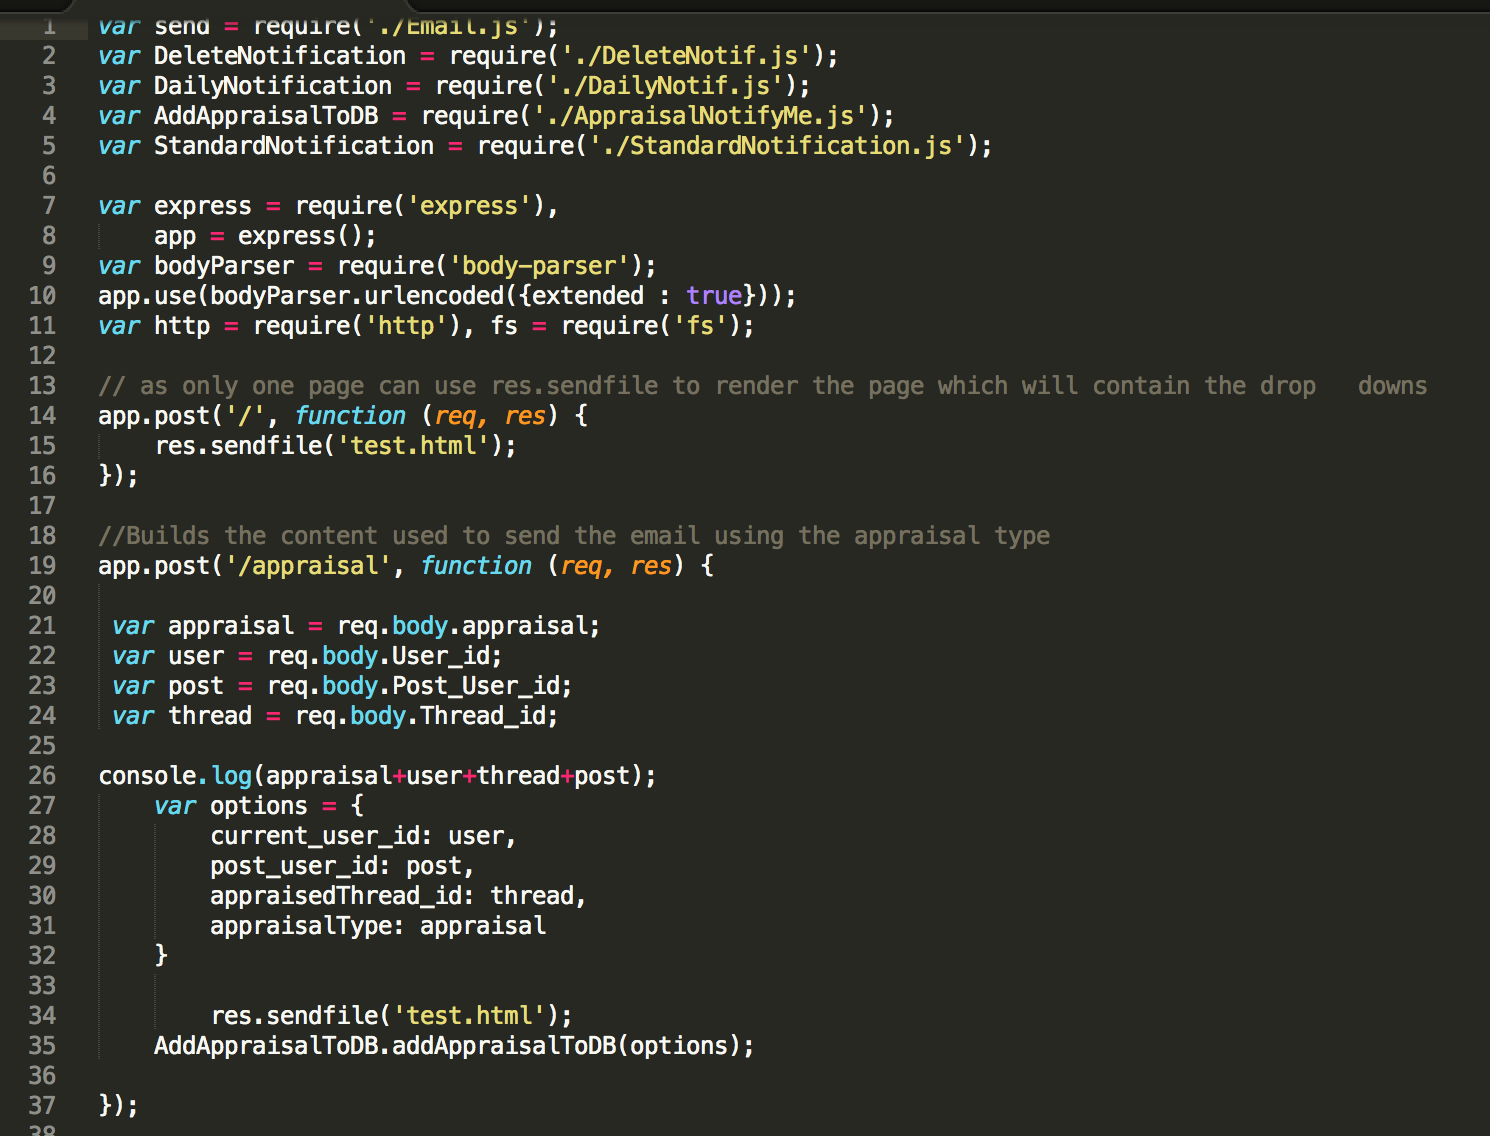
\includegraphics[width=1.0\textwidth]{IntegrationUnitTest}}
			\caption{Unit Tests}
			\label{fig:scope}
		\end{figure}
	\item database issues
	There is no way to access the specified database and this also contributes to the integratability. They should supply a way to specify the database to be used.
		~\ref{fig:IntegrationDatabaseFail}
		\begin{figure}[H]
			\centering
			\fbox{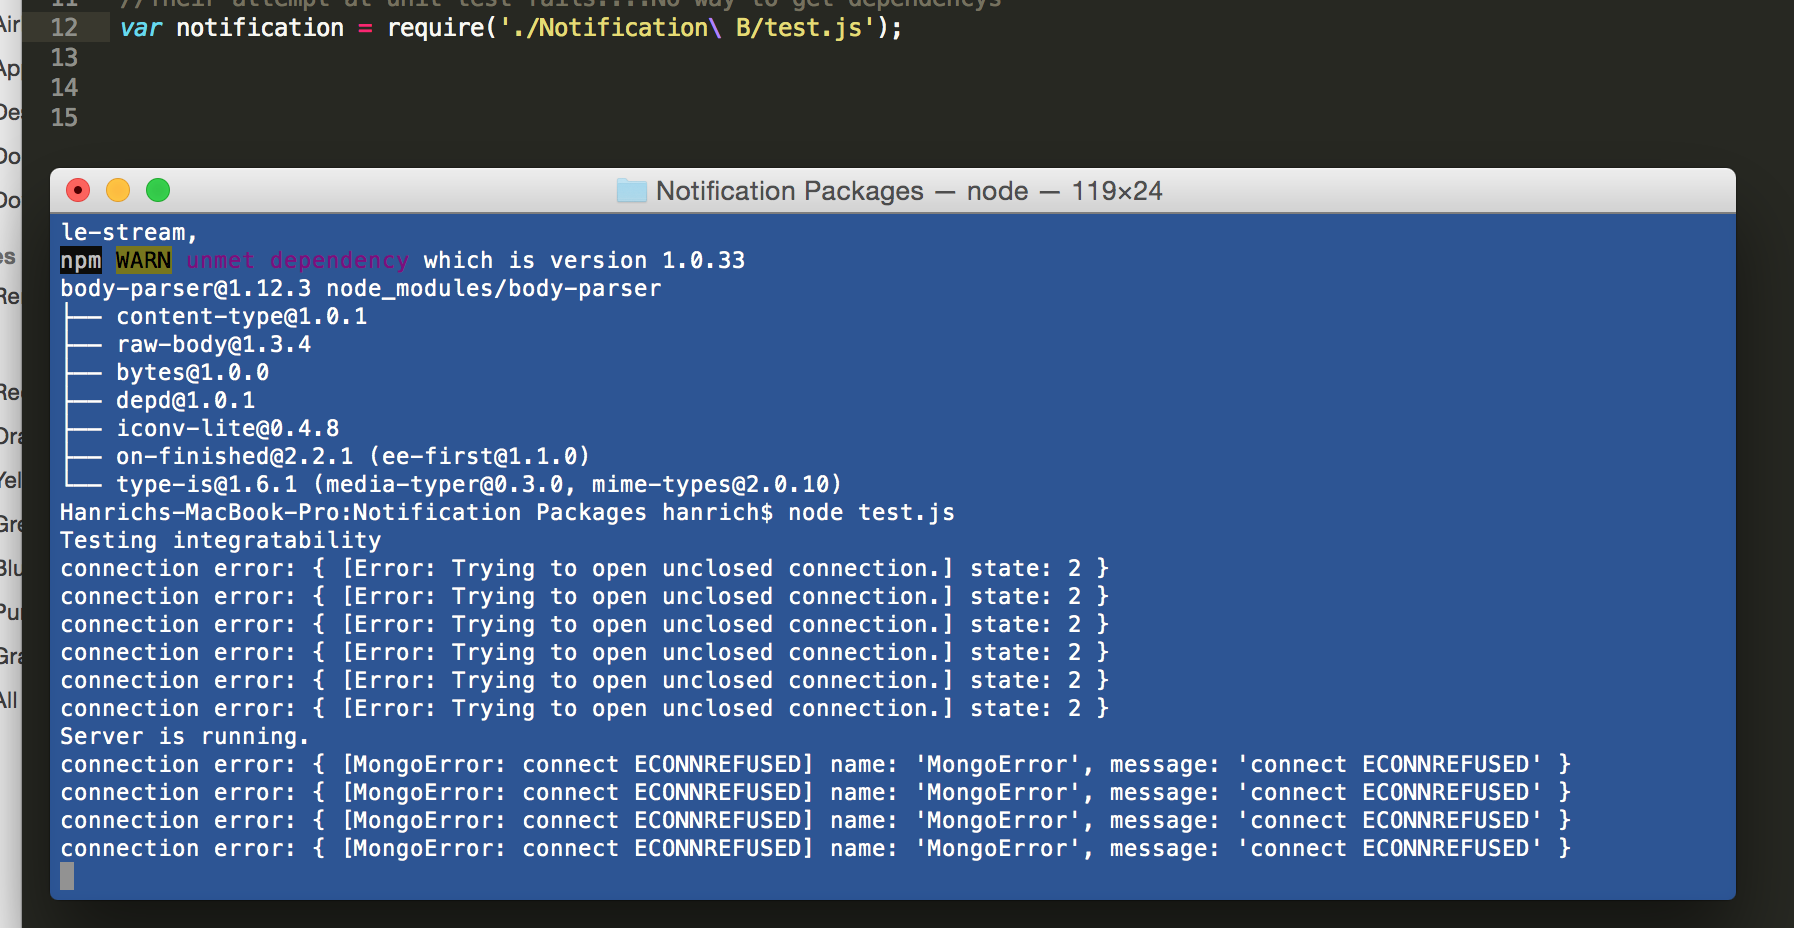
\includegraphics[width=1.0\textwidth]{IntegrationDatabaseFail}}
			\caption{Database connection issues}
			\label{fig:scope}
		\end{figure}
Both modules suffer from common symptoms when it comes to Integratability. I therfore conclude that neither system is integratable and needs to look at dependancy injection. Each package should at least include a npm readme file to specify the packages are required.
\end{itemize}
\subsubsection*{Remarks}
Notification B is not Integratable at all. There is no provision for dependancy injection.